\chapter{ARIA: System architecture}
The selected system is a compromise between payload capacity, in-flight stability and
manoeuvrability and low-cost. The system is composed by:
\begin{itemize}
    \item Tarot 650 Sport drone, for the platform
    \item Hex Cube Black Flight Controller
    \item HERE2 GPS system
    \item Raspberry Pi3b+ for the controller devoted to sensor measurement
    \item A suite of sensors for air quality monitoring (in particular NO, NO2, CO and VOCs) based on Alphasesnse AFE board
    \item Nova SDS011 PM board to measure PM2.5 and PM10
    \item Taranis 9D+ Radio and an 8XR receiver
\end{itemize}
\begin{figure}[h!]
    \centering
    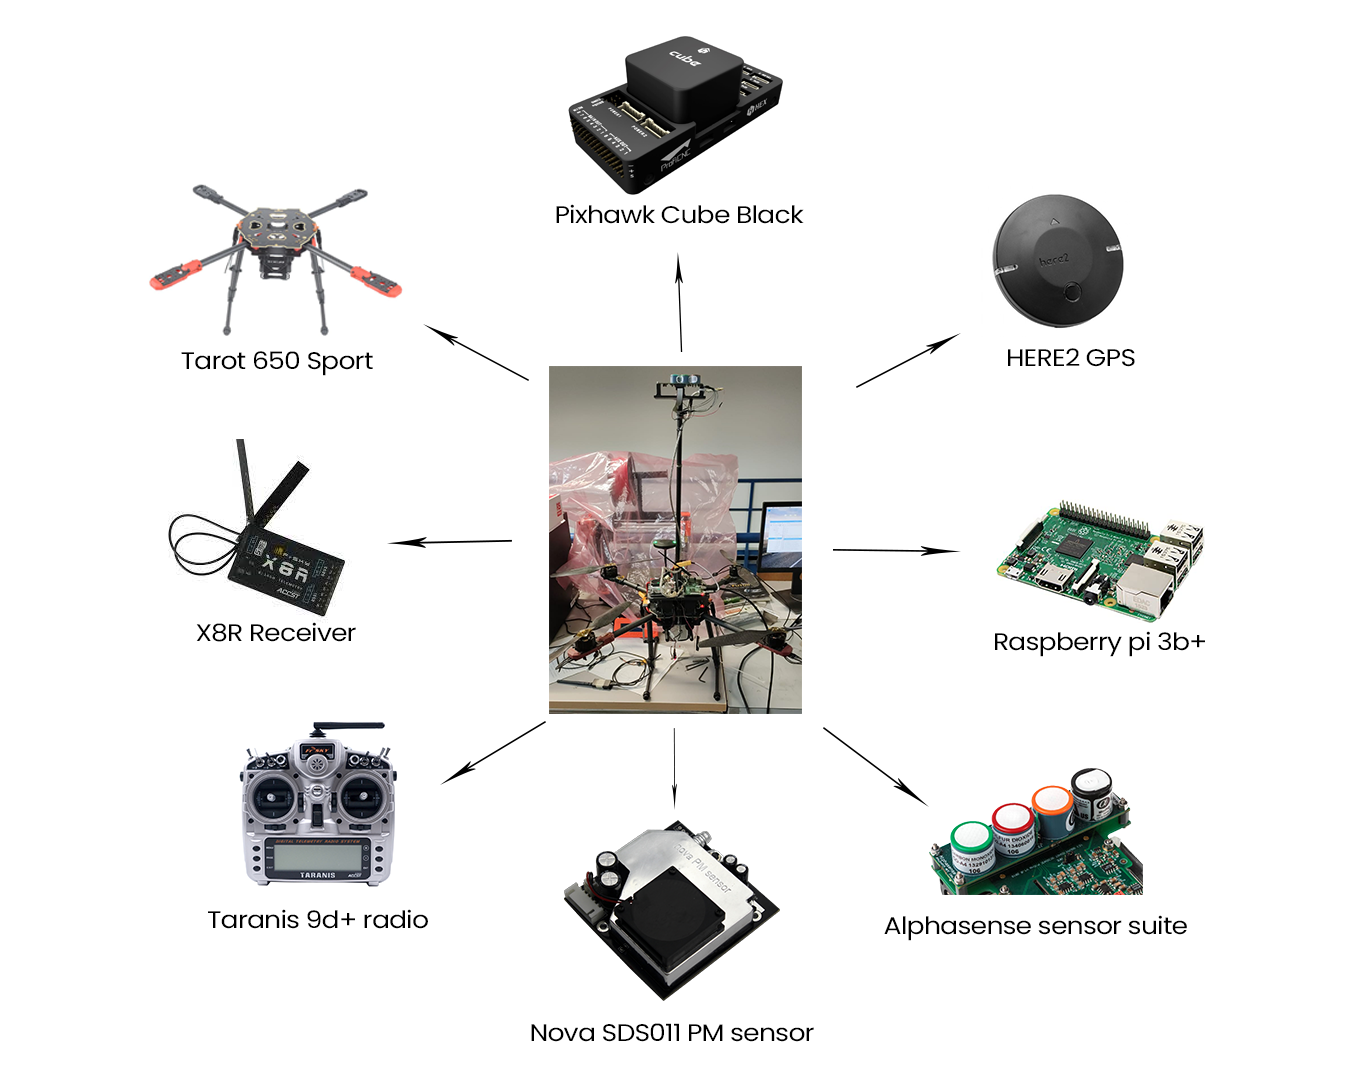
\includegraphics[width=1\textwidth]{images/system-architecture.png}
    \caption{\gls{aria} drone system components}
    \label{fig:aria-drone}
\end{figure}
The ARIA Project is going to use
simultaneously two drones and a fixed ground station, equipped with the same instrumentation in
order two build a 3D map of the investigated area. We are currently experimenting with the use of an Arduino controller on the second drone to compare the data collected by a different platform and allow the presence of additional sensor (such as temperature) thanks to Arduino's support of an higher number of input channels. This dissertation will focus on the Rapberry based system.
There has been just some laboratory testing on the effect of the blade disturbances on the measurement \cite{8453584}
but a comprehensive study on sensor location on such platforms has not been done yet; therefore
the ARIA project has designed a vertical boom were all the gas sensors are located. On the other
hand, in the area above the UAV, there is a relatively constant air flow which drops significantly after
a distance of approximately 40.0-50.0 cm for devices with characteristics similar to those used in the
proposed solution. The airflow behaviour is similar aside from the UAV in the area with a radius from
the center r $>$ 50.0 cm. To avoid the swirl area, it is recommended to place horizontal and vertical
probes of the appropriate length. The use of horizontal probes often makes it difficult to achieve the
conditions necessary for isokinetic sampling. In addition, it is necessary to use additional structures for their equalization. To overcome this problem, it was decided to use the vertical probe; the use of a
boom in a vertical position does not affect the flight capabilities of the UAV since the entire system has
a low center of mass, situated in the proximity of the battery.
Figure \ref{fig:aria-drone} contains an overview of the various system components; while Figure \ref{fig:system} shows one of the drones and some details of the system.
The UAV pilot or the UAV \gls{gso} can communicate with the UAV
wirelessly, using a radio controller (RC) transmitter or a computer, respectively.
Power is provided by a 6s Lipo battery able to give 10000mAh. Communication
between the flight controller and ground station is via 433MHz telemetry link connected to a laptop; a
2.4GHz communication link is also ensured via the Taranis 9D+ Radio and an 8XR receiver onboard the
UAV.
\clearpage
\begin{figure}[!ht]
    \centering
    \begin{subfigure}[b]{0.32\textwidth}
        \centering
        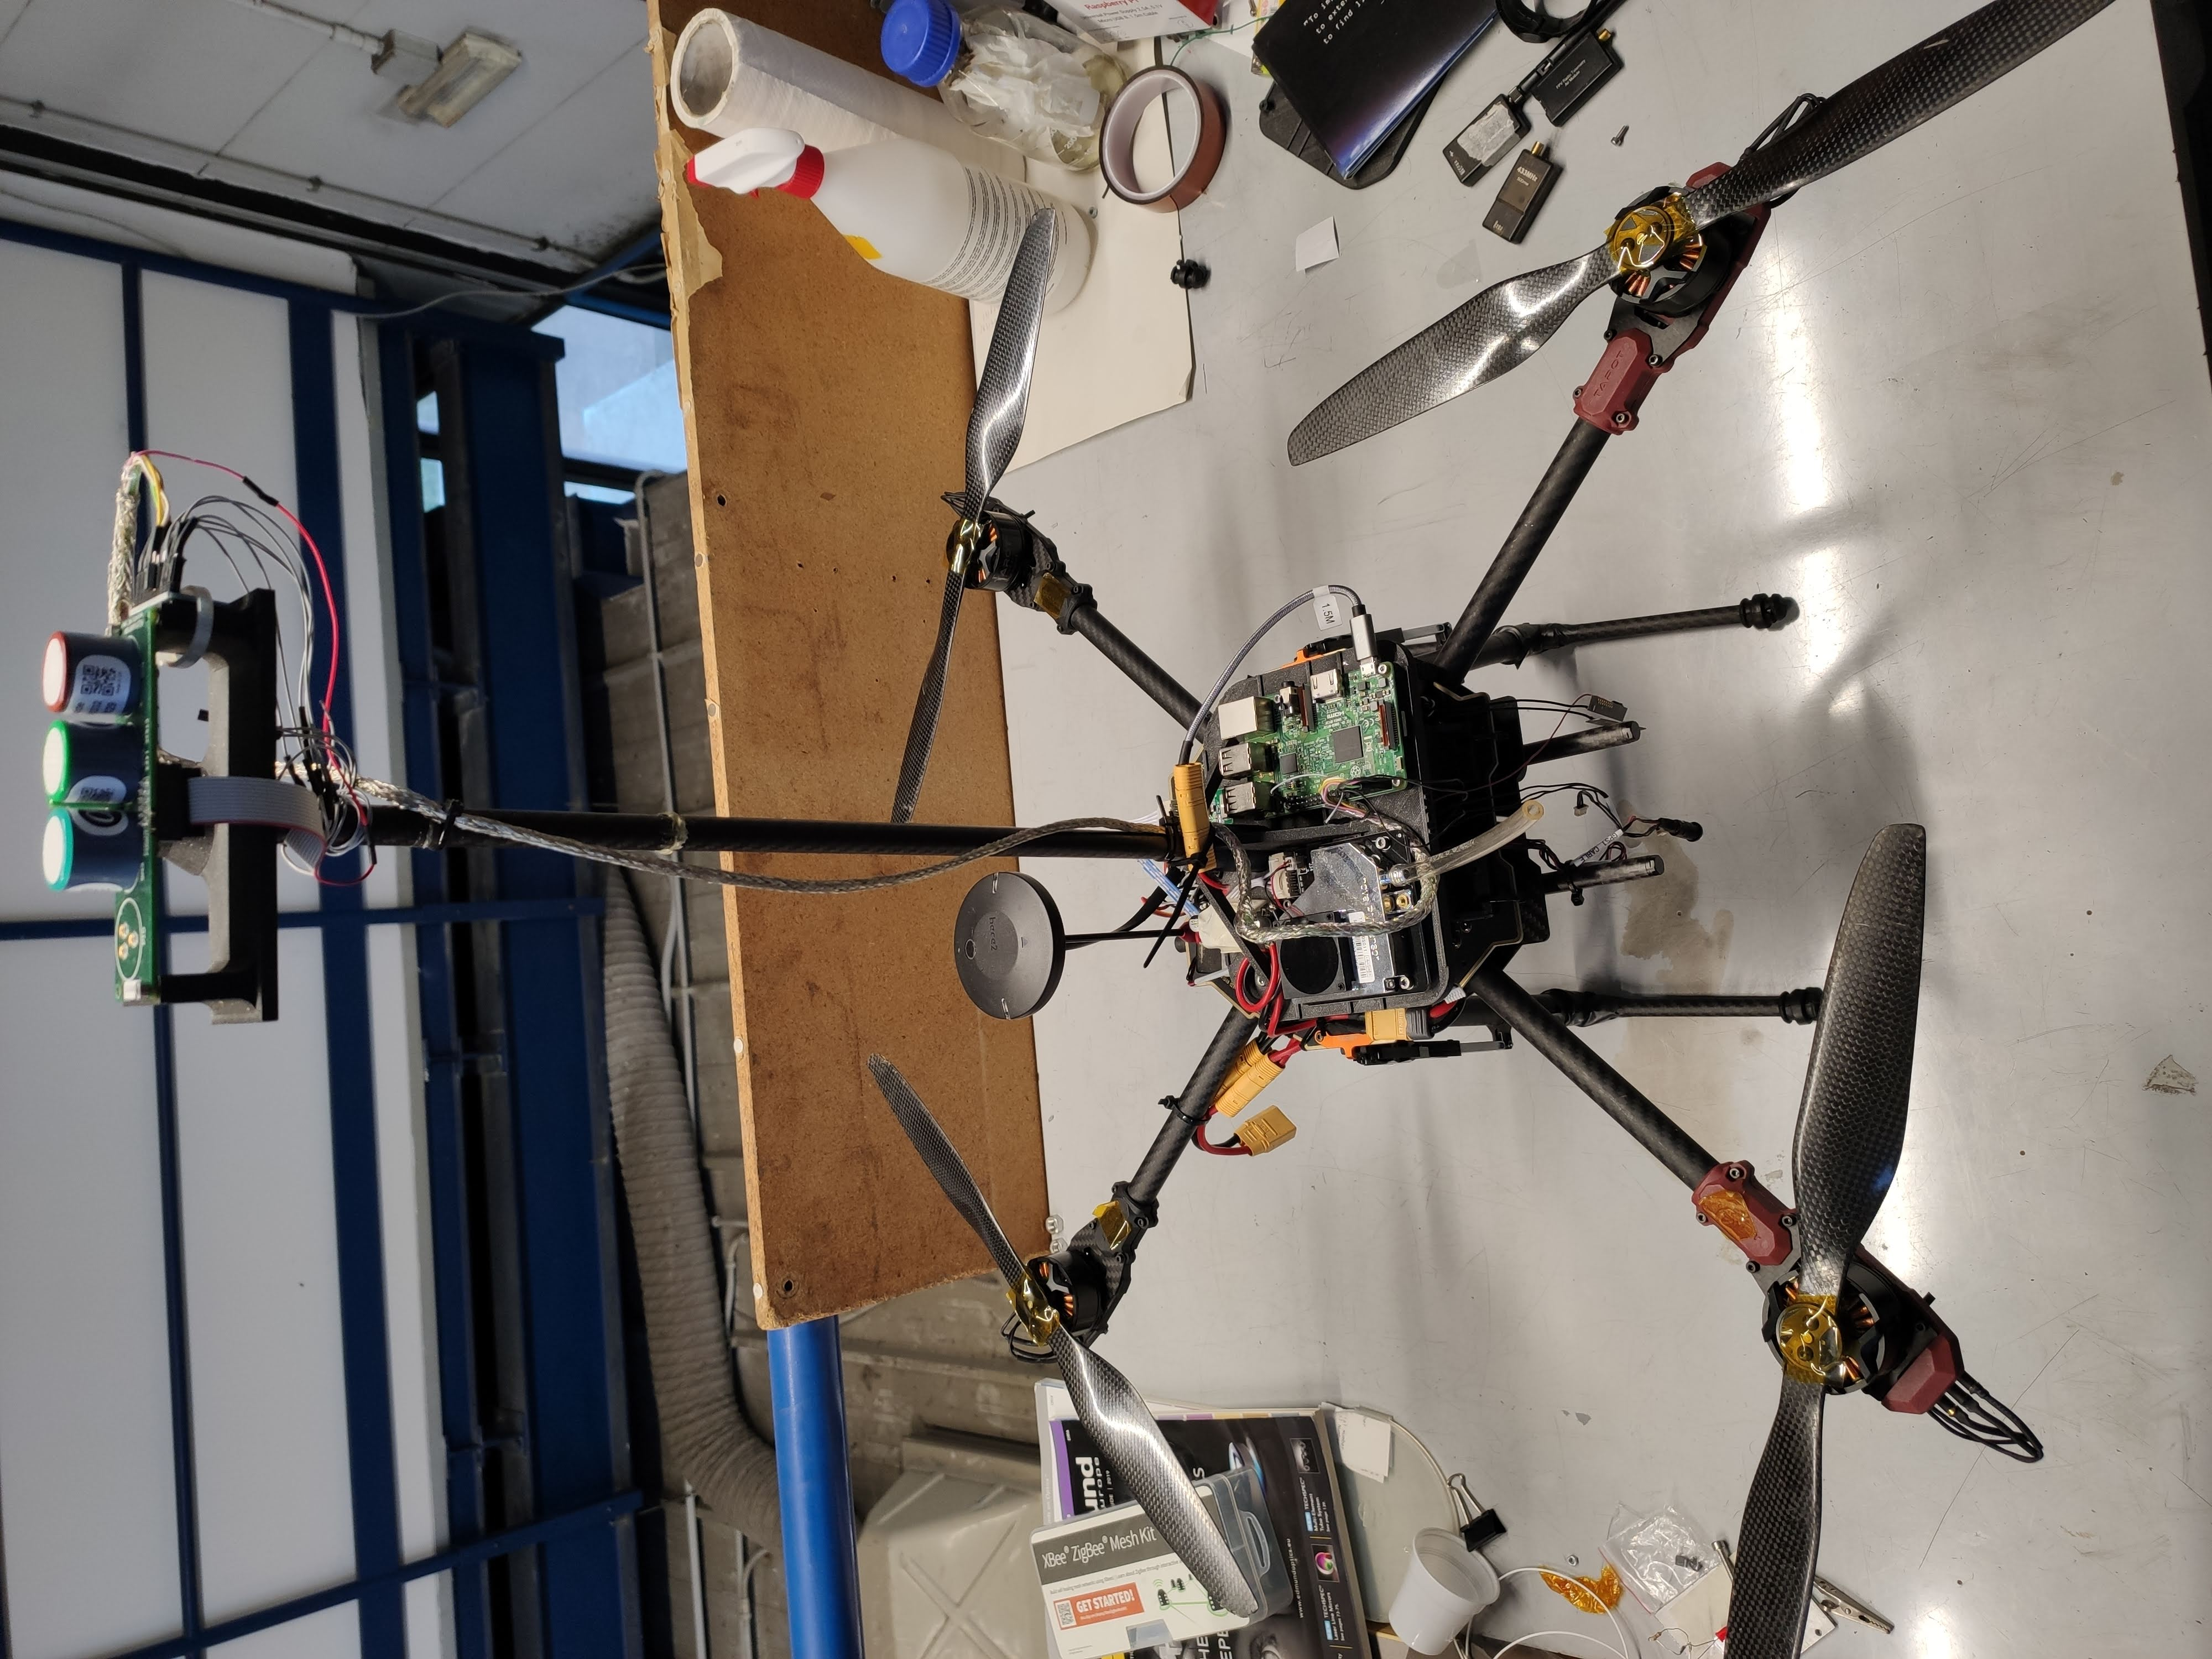
\includegraphics[width=\textwidth, angle=-90]{images/drone/IMG_20211105_103832.jpg}
        \caption{}
        \label{fig:wide}
    \end{subfigure}
    \begin{subfigure}[b]{0.32\textwidth}
        \centering
        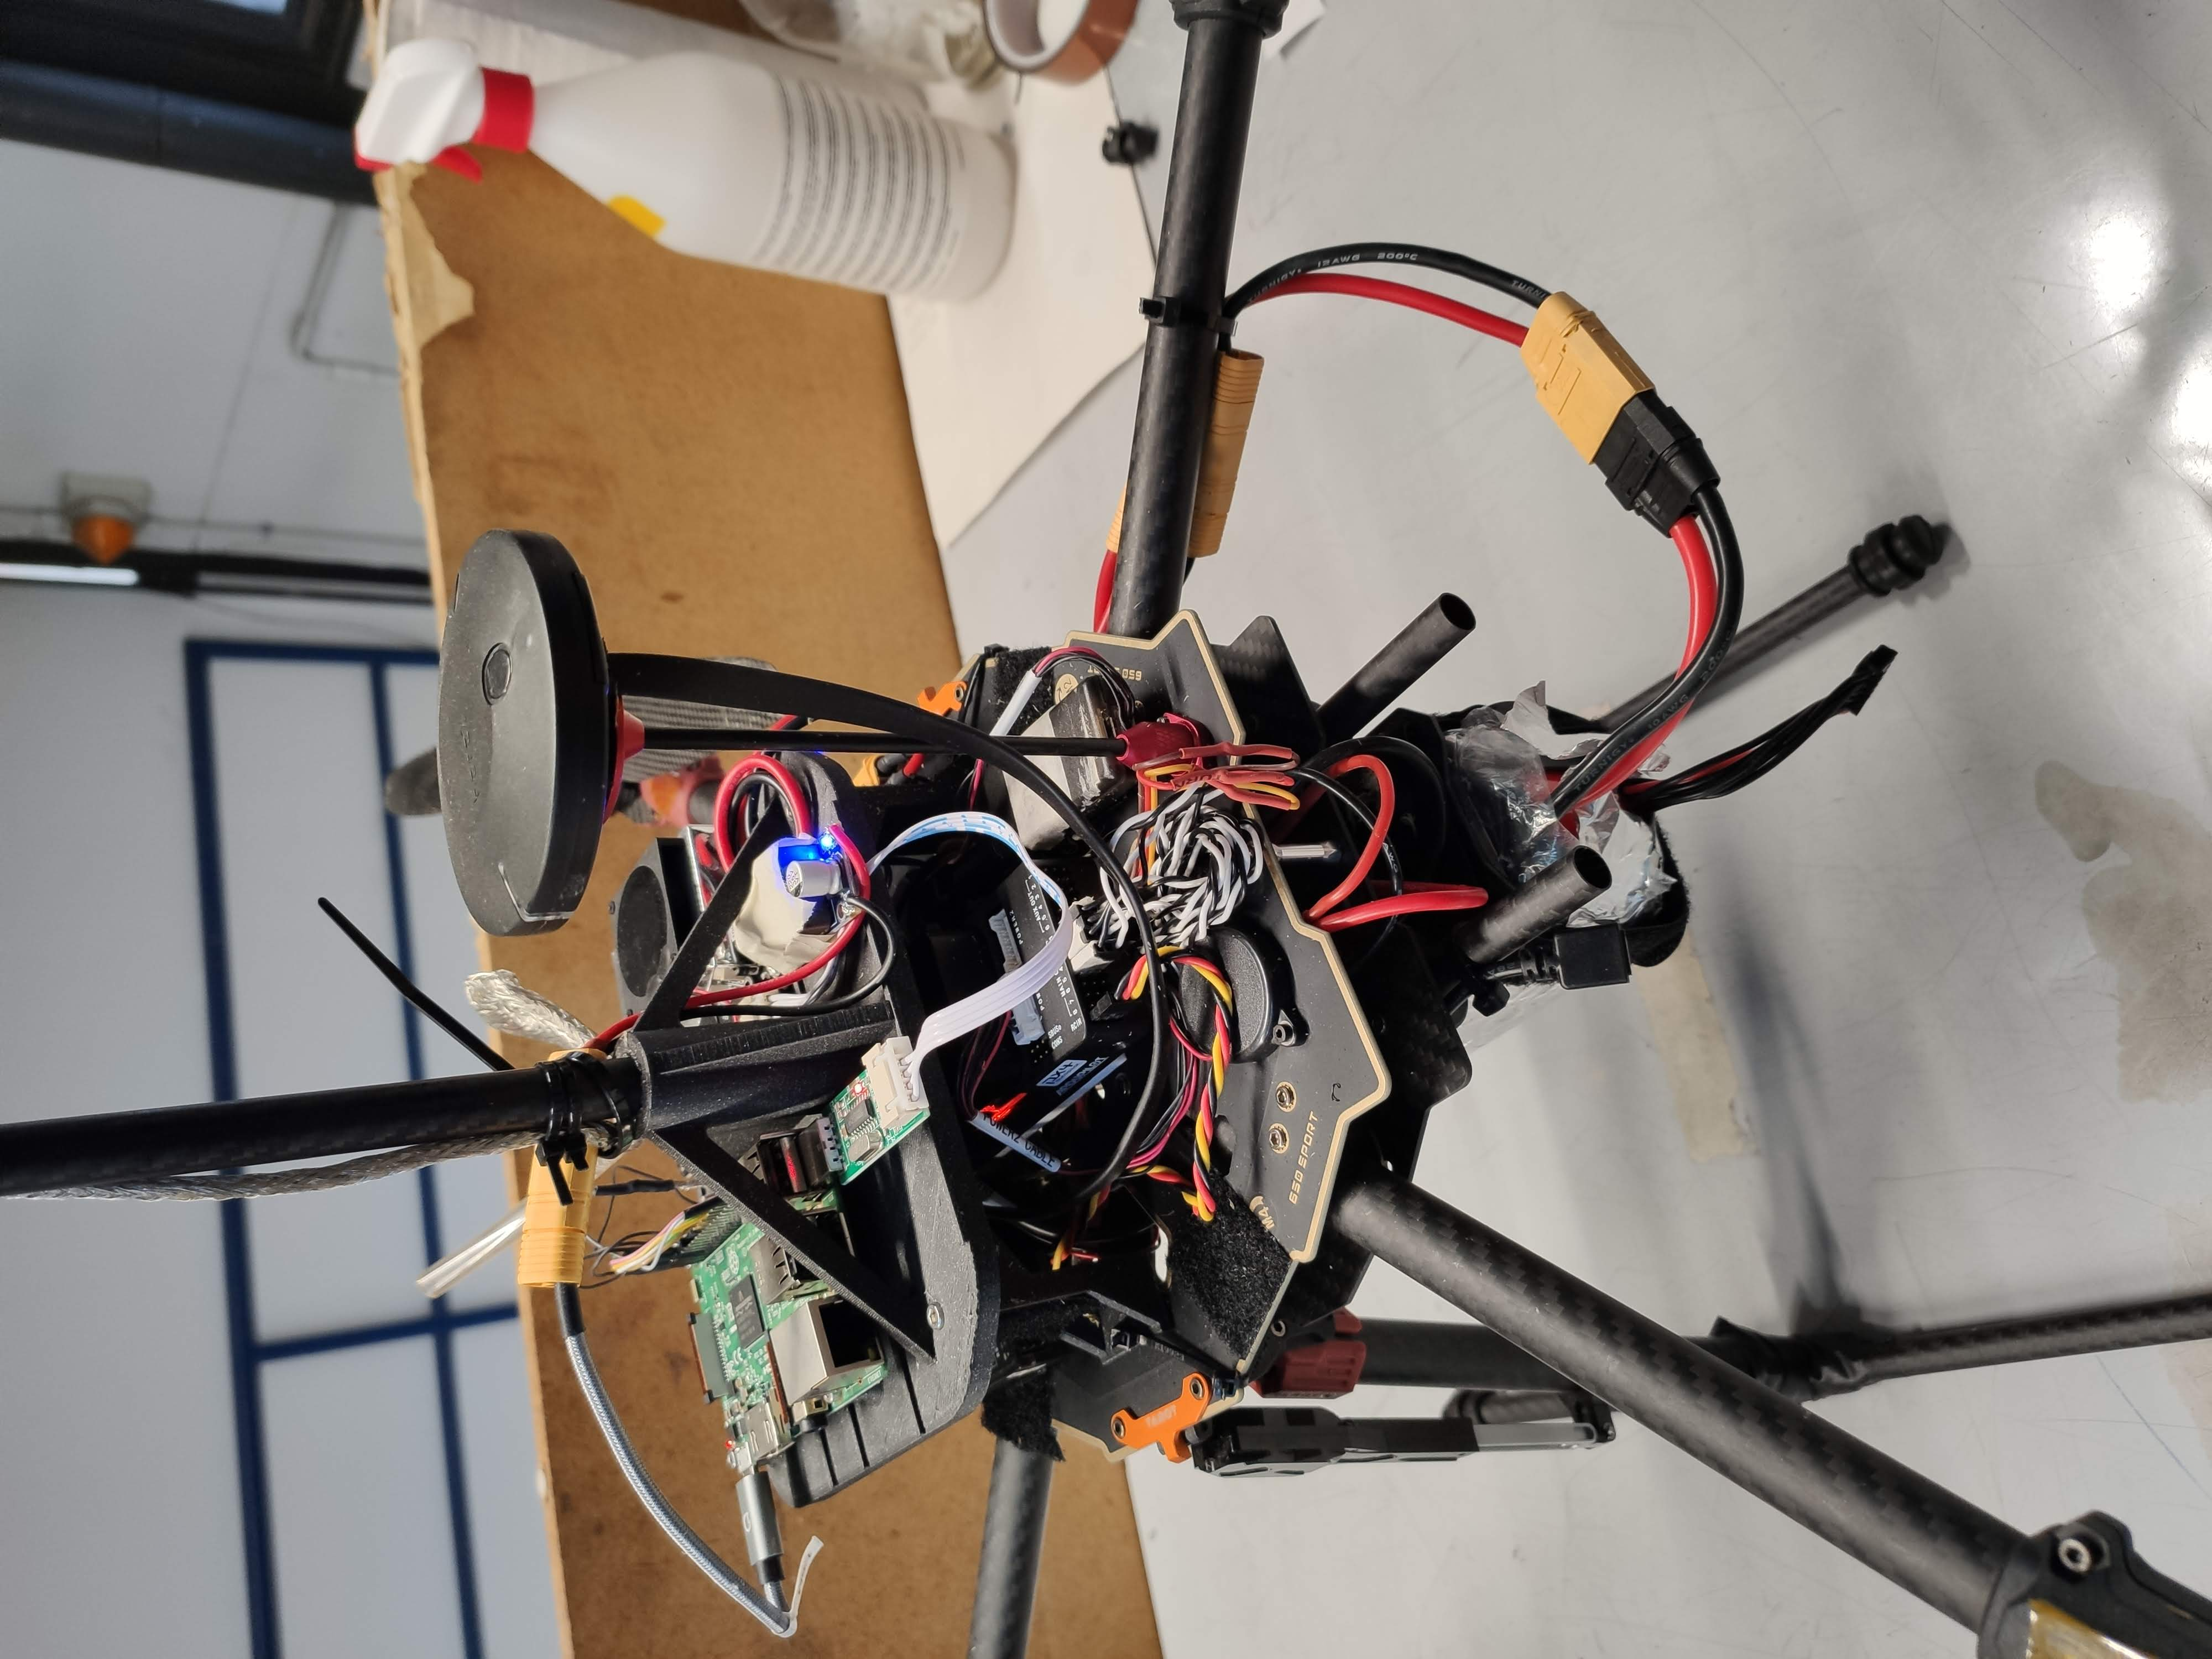
\includegraphics[width=\textwidth, angle=-90]{images/drone/IMG_20211105_103729.jpg}
        \caption{}
        \label{fig:auto}
    \end{subfigure}
    \begin{subfigure}[b]{0.32\textwidth}
        \centering
        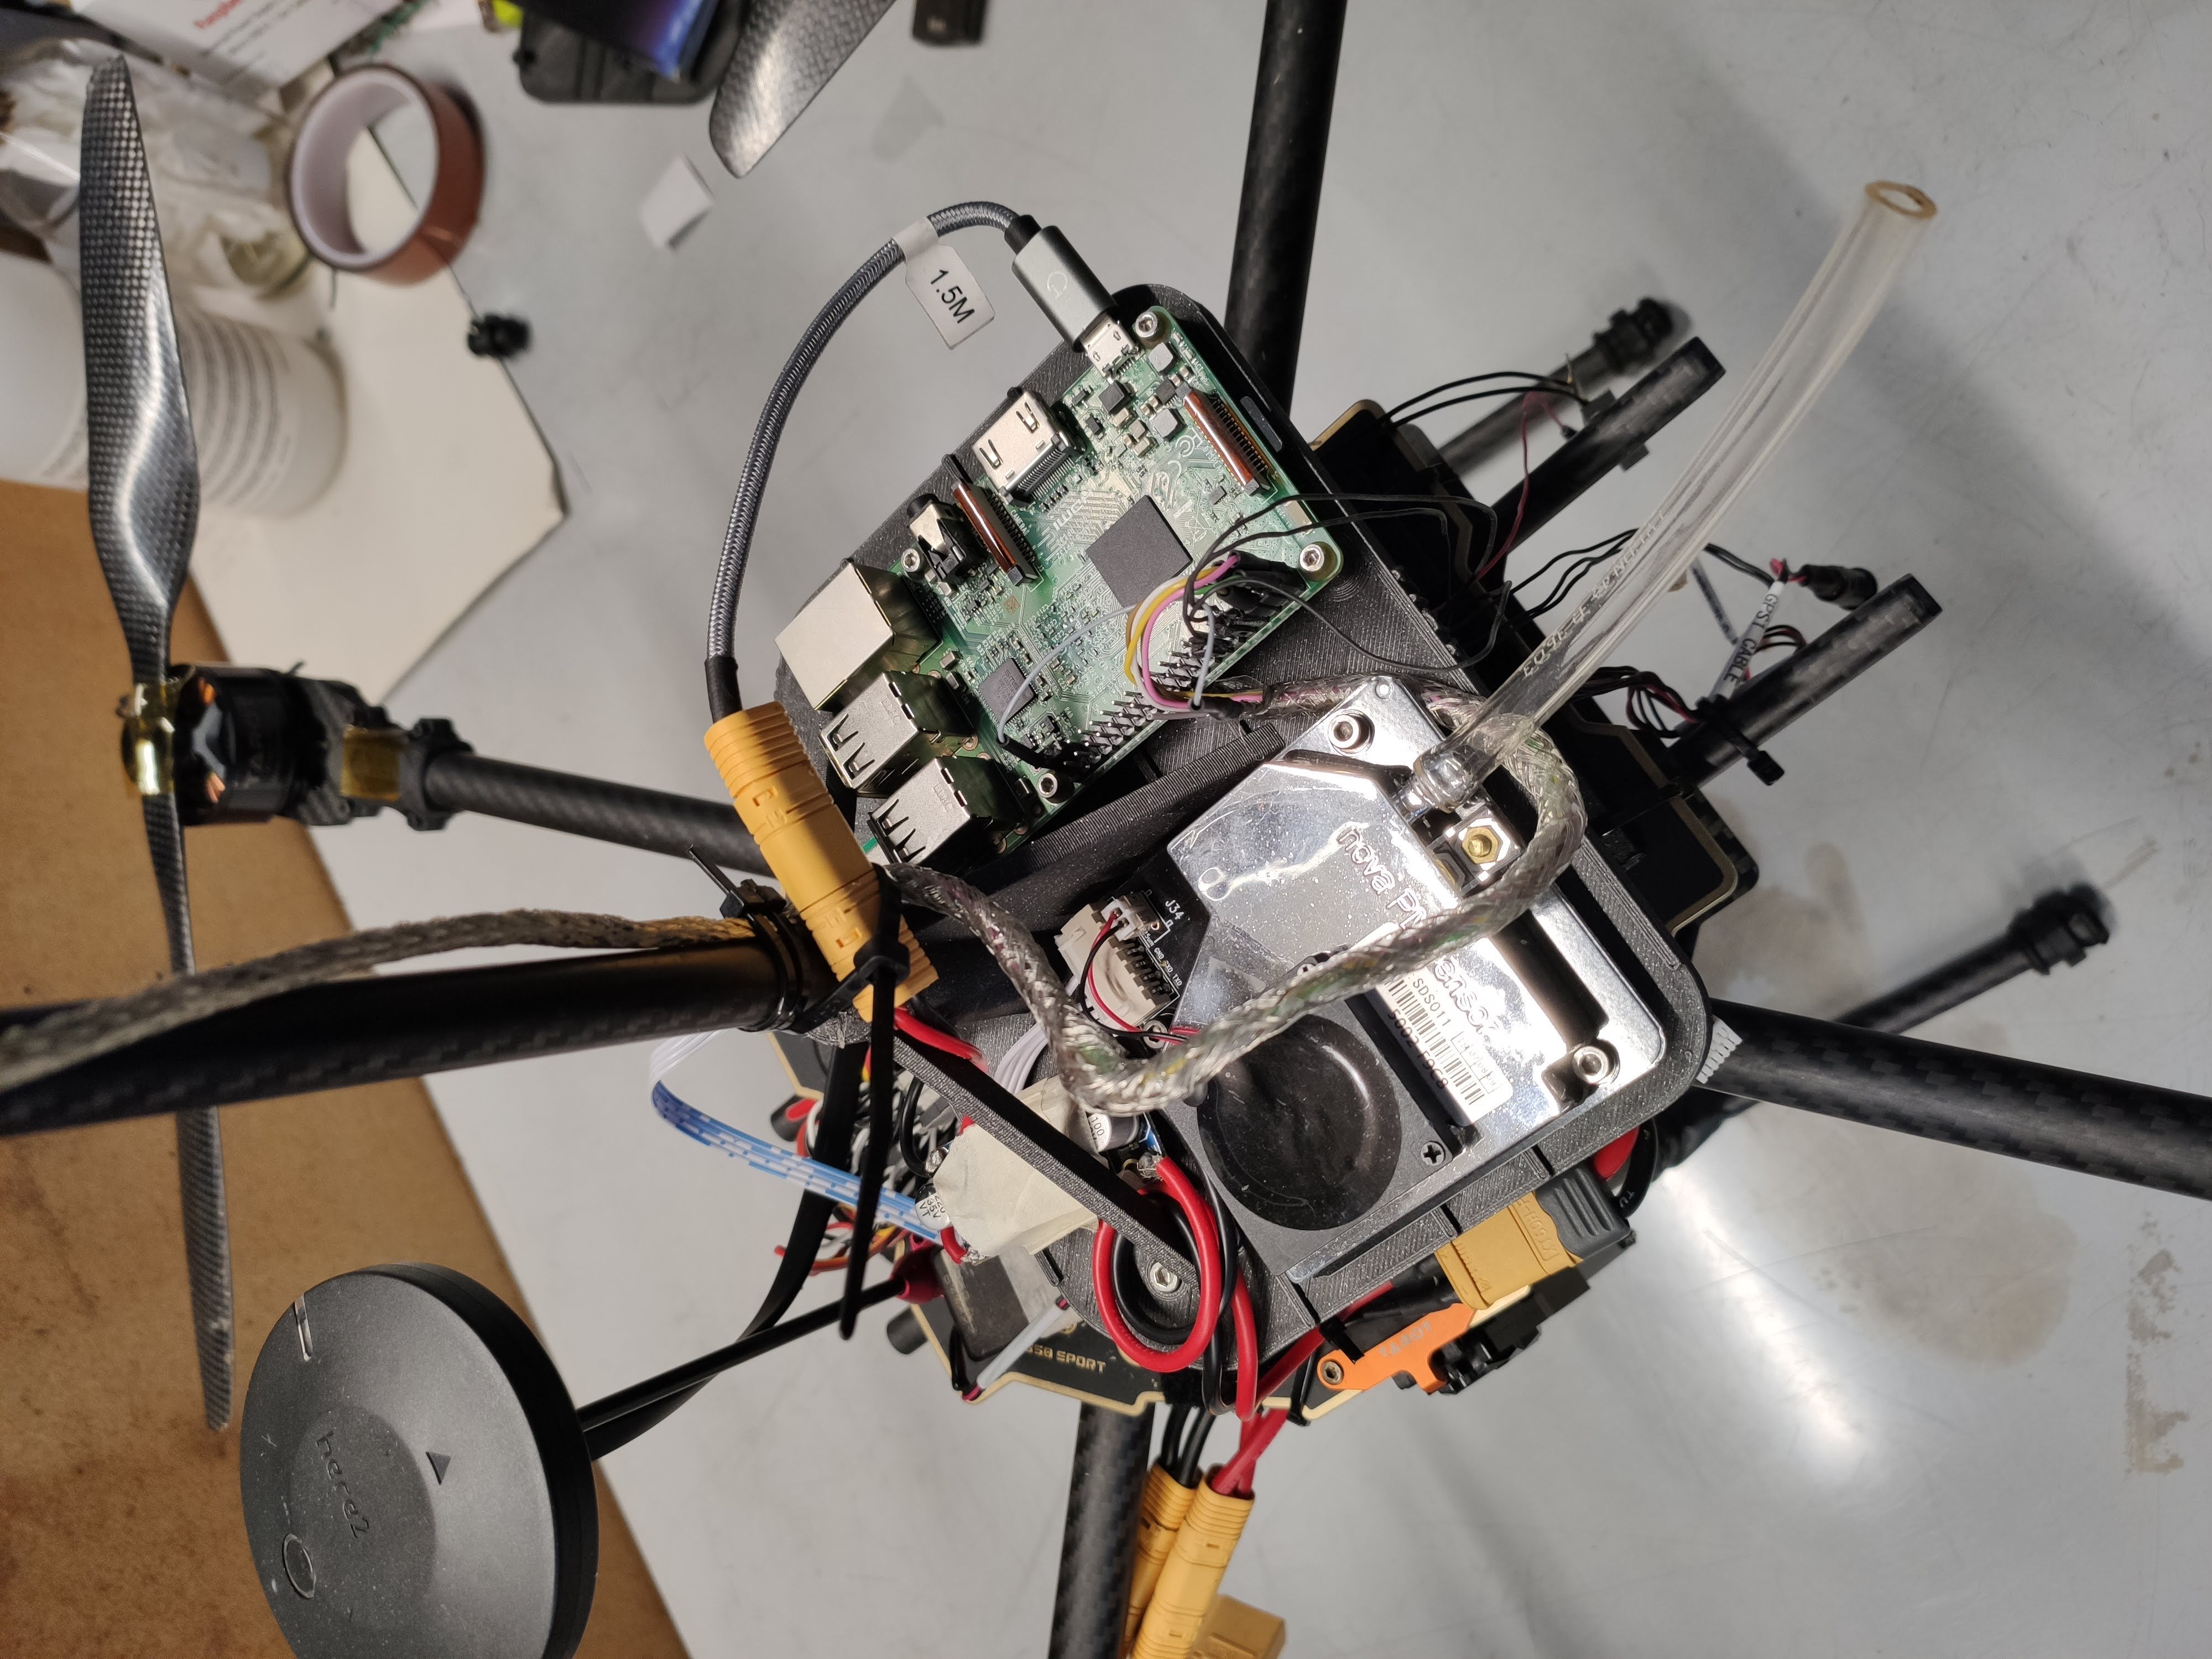
\includegraphics[width=\textwidth, angle=-90]{images/drone/IMG_20211105_103839.jpg}
        \caption{}
        \label{fig:rasp}
    \end{subfigure}
       \caption{The Rasperry Pi \gls{aria} drone}
       \label{fig:system}
\end{figure}
